\section{镜 (45pts)}
如图\ref{mirror} 所示,这道题是三个简单的几何光学问题。所有镜子的距离是\(d\),焦距是\(f\)或者\(-f\),设第一个物距为\(u\),请你回答下面的问题:
\begin{figure}[htbp]
	\centering
	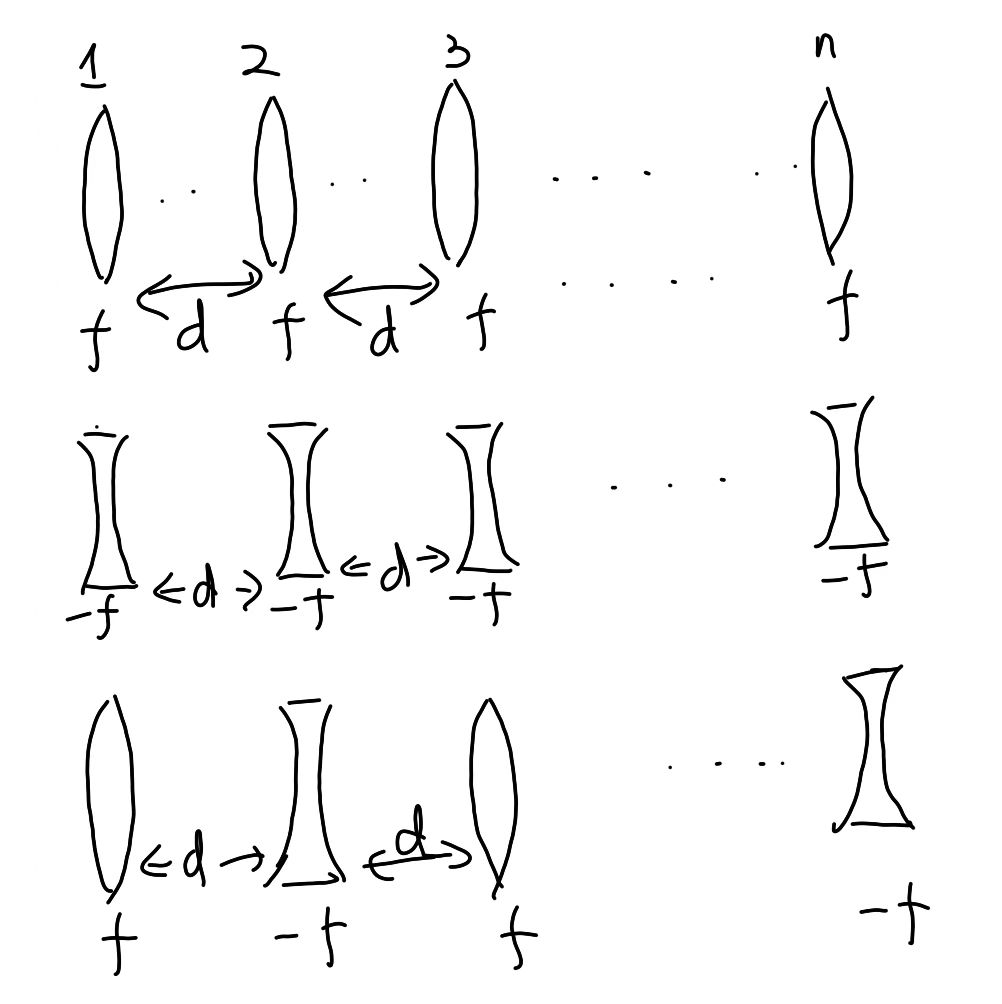
\includegraphics[width=0.5\textwidth]{mirror}
	\caption{这是三道摆放方案.}
	\label{mirror}
\end{figure}
\begin{enumerate}
	\item 光路全由凸透镜构成,总共\(n\)个凸透镜,求出最后的像距\(v\)与物距\(u\)的关系式。提示:你需要分两种情况讨论:\(d=4f\), \(d\neq 4f\)。 (30pts)
	\item 光路全由凹透镜构成,总共\(n\)个凹透镜,求出最后的像距\(v\)与物距\(u\)的关系式。(5pts)
	\item 光路全由凹透镜和凸透镜交替构成,总共\(n\)个透镜,得出相邻两项递推关系式给出计算方法即可(需要确保可以实现),无需给出具体答案(10pts) 
\end{enumerate}

\section*{Answer 5}
\begin{enumerate}
	\item 有成像公式:
	\begin{align*}
		\frac{1}{f} &= \frac{1}{u} + \frac{1}{v} \\
		v &= \frac{fu}{u-f}\\
		u_{n} & = d-v_n \\
		v_n &= \frac{fu_{n}}{u_{n}-f} 
	\end{align*}
	可以填充定义:
	\begin{align*}
		v_0 = d - u
	\end{align*}
	递推关系为:
	\begin{align*}
		v_{n+1} &= \frac{(d-v_n)f}{d-v_n-f} 
	\end{align*}
	使用不动点法,令\(v_{n+1} = v_n = x\),得到:
	\begin{align*}
		x^2 -  xd + fd &= 0 
	\end{align*}
	当\(d=4f\)的时候,只有一个解:
	\begin{align*}
		x = \frac{d}{2} = 2f
	\end{align*}
	此时我们做一下数学变换:
	\begin{align*}
		v_{n+1} - 2f &= \frac{v_n - 2f}{3f - v_n}f \\
		\frac{f}{v_{n+1} - 2f} &= \frac{3f - v_n}{v_n - 2f} = \frac{f}{v_n - 2f} - 1 
	\end{align*}
	发现为等差数列,立即递推得出:
	\begin{align*}
		\frac{f}{v_{n} - 2f} &= \frac{f}{v_0 -2f} - n 
	\end{align*}
	由此可得:
	\begin{align*}
		v = v_n = 2f + \frac{f}{\frac{f}{2f - u} - n} 
	\end{align*}
	当\(d \neq 4f\)的时候,有两个解(不论是实数还是复数均可以):
	\begin{align*}
		&x_1 x_2 = fd \\
		&x_1 + x_2 = d 
	\end{align*}
	对递推关系做变换:
	\begin{align*}
		v_{n+1} -x_1 &= \frac{(d-v_n)f}{d-v_n-f} - x_1 \\
		&= \frac{df - v_n f - x_1 d - v_n x_1 - f x_1}{d-v_n-f} \\
		&= \frac{(v_1 - x_1 )(x_1 -f )}{d-v_n-f} \\
		v_{n+1} - x_2 &= \frac{(v_1 - x_2 )(x_2 -f )}{d-v_n-f} \\
	\end{align*}
	两式相除,得到:
	\begin{align*}
		\frac{v_{n+1} - x_1}{v_{n+1} - x_2} &= \frac{(v_n - x_1 )(x_1 -f )}{(v_n - x_2 )(x_2 -f )} 
	\end{align*}
	发现为等比数列,于是立即递推得出:
	\begin{align*}
		\frac{v_{n} - x_1}{v_{n} - x_2} &= \frac{v_0 - x_1}{v_0 - x_2} \prod_{i=0}^{n-1} \frac{x_1 -f}{x_2 -f} \\
		&= \frac{v_0 - x_1}{v_0 - x_2} \left(\frac{x_1 -f}{x_2 -f}\right)^n 
	\end{align*}
	从而得到:
	\begin{align*}
		v_n &=\frac{x_1 + \frac{v_0 - x_1}{v_0 - x_2} \left(\frac{x_1 -f}{x_2 -f}\right)^n x_2}{1+ \frac{v_0 - x_1}{v_0 - x_2} \left(\frac{x_1 -f}{x_2 -f}\right)^n} 
	\end{align*}
	带入\(v=v_n, v_0 = d-u\),得到:
	\begin{align*}
		v &= \frac{x_1 + \frac{d-u - x_1}{d-u - x_2} \left(\frac{x_1 -f}{x_2 -f}\right)^n x_2}{1+ \frac{d-u - x_1}{d-u - x_2} \left(\frac{x_1 -f}{x_2 -f}\right)^n} 
	\end{align*}
	\item 这里注意到只需要将\(f\)换成\(-f\)即可,并且注意到了此时将不会有分类讨论的情况,因为距离永远是大于0的。
	\begin{align*}
		v &= \frac{x_1 + \frac{d-u - x_1}{d-u - x_2} \left(\frac{x_1 +f}{x_2 +f}\right)^n x_2}{1+ \frac{d-u - x_1}{d-u - x_2} \left(\frac{x_1 +f}{x_2 +f}\right)^n} 
	\end{align*}
	\item 此时我们仍从递推关系出发:(令\(v_0 = d-u\))
	\begin{align*}
		\frac{1}{d-v_0} + \frac{1}{v_1} &= \frac{1}{f} \\
		\frac{1}{d-v_1} + \frac{1}{v_2} &= \frac{1}{-f}
	\end{align*}
	此时的相邻的递推需要是角标差为2的关系式:
	\begin{align*}
		v_2 = \frac{(d^2 - 2df + (f-d)v_0)(-f)}{d^2-df-f^2-dv_0}
	\end{align*}
	不难发现我们仍然可以使用不动点发做,然后同第一小问一样的解法即可。

\end{enumerate}